% \documentclass{report}

% \usepackage{fancyhdr}
\usepackage{fourier-orns}
\usepackage{hyperref}%% To refrence links / jumps
\usepackage{chngcntr} %% For some extra counters numberings
\usepackage[a4paper, right = 0.5in, left = 0.5in,top = 1in , bottom = 1in]{geometry}
\usepackage{etoolbox} %% Provides like a language for advanced customization
\usepackage{datetime} %% For dates of course
\usepackage{lastpage} %% provides pages numbers
\usepackage[sc]{titlesec} %% modify titles
\usepackage{enumerate}
\usepackage{cancel}
\usepackage{tikzsymbols}
\usepackage[dvipsnames]{xcolor}
\usepackage{import}
\usepackage{pdfpages} %% include other pdfs
\usepackage{transparent} %% Transparency
\usepackage{xcolor}  %% Colors
\usepackage[many]{tcolorbox}
\usepackage[framemethod=TikZ]{mdframed}
\usepackage{amsmath,amsfonts,amsthm,amssymb,mathtools}
\usepackage{tikz}
\usepackage{bookmark}
\usepackage{graphicx}
\usepackage{mathpazo}

\usepackage{fontawesome5}

\linespread{1.5}


\titleformat{\chapter}[display]   
{\fontfamily{ppl}\selectfont\huge\color{YellowOrange!80!orange}} % Font style and size 
{\raggedleft\color{purple}\fontsize{70}{0pt}\selectfont\thechapter}   
{-1.5cm}    			                          % Space between the chapter number and title
{
	\begin{tikzpicture}[overlay]
		\node[anchor = west,yshift = 0.2cm,xshift = -1cm] {\fontsize{90}{20} $\int_{}^{} $};
		\node[yshift = 4cm, xshift = 17cm]   {\includegraphics[width = 4cm]{preview0}};
	\end{tikzpicture}
\hspace{1cm}\Huge\raggedright\MakeUppercase}

\titleformat{\section}[block]
{
\fontfamily{ppl}\selectfont\huge\color{YellowOrange!80!orange}
}
{
\color{purple}\fontsize{20}{0pt}\selectfont\thesection 
}
{0cm}
{
	\begin{tikzpicture}[overlay]
		\node[anchor = west,yshift = 0.2cm,xshift = -0.4cm, circle = 1pt] {};
	\end{tikzpicture}
}

\titlespacing*{\section}{0pt}{0.7cm}{1.5cm}


\newcommand{\divider}
{
	\begin{center}
	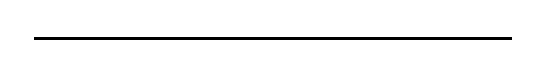
\begin{tikzpicture}
		\draw[thick, black] (0.25*\textwidth, 0) -- (0.75*\textwidth, 0);
		\node[rotate = 360 - 90, xshift = -0.6pt, yshift = 1pt] at (0.25*\textwidth,0){\decotwo};
		\node[rotate = 90, xshift = -0.6pt, yshift = 1pt] at (0.75*\textwidth,0){\decotwo};
	\end{tikzpicture}
	\end{center}
}

\pagestyle{fancy}

\newcommand{\lecday}[1][]
{
    \def\datee{#1}
    \fancyhead[L]{\datee}
}



\newcommand{\signature}
{
	\begin{tikzpicture}[remember picture,overlay]
		\node[fill = YellowOrange!20!white] at ([yshift = 1cm, xshift = -3cm]current page.south east) {\fontsize{10pt}{0pt}{\itshape Kara.$\mathcal{A}$}};
	\end{tikzpicture}
}

\AddToHook{shipout/background}{
  \begin{tikzpicture}[remember picture, overlay]
	  \node[] at ([yshift = 1.5cm,xshift = \textwidth /2 + 0.9cm]current page.south west) {\includegraphics[width = 0.5cm]{preview3}};
	  \node[] at ([yshift = 1.5cm,xshift = - \textwidth /2 - 0.9cm]current page.south east) {\includegraphics[width = 0.5cm]{preview4}};
  \end{tikzpicture}
}



\newtcolorbox[auto counter, number within = section]{remark}[1][]
{
       		title = Remark #1,
		enhanced,
		boxrule = 0pt,
		colback = white,
		breakable,
		arc = 4pt,
		colbacktitle = cyan,
		colback = cyan!5!white,
		segmentation style =
		{
			solid,cyan,thick,
		},
		attach boxed title to top left =
		{
			xshift = 0cm,
		},
		boxed title style =
		{
			boxrule = 0pt,
			sharp corners,
			drop fuzzy shadow = {cyan},
		},
		drop fuzzy shadow = {cyan!80!black},
}

\newtcolorbox[auto counter, number within = section]{theorem}[1][]
{                                      
		title = Theorem \thetcbcounter : #1,
		enhanced, 
		boxrule = 0pt,
		colback = white,
		breakable,
		arc = 4pt,
		colbacktitle = purple,
		colback = purple!5!white,
		segmentation style = 
		{
			solid, purple,thick,
		},
		attach boxed title to top left = 
		{
			xshift = 0cm, 
		},
		boxed title style = 
		{
			boxrule = 0pt,
			sharp corners,
			drop fuzzy shadow = {purple},
		},
		drop fuzzy shadow = {purple!80!black},
}

\newtcolorbox[auto counter, number within = section]{definition}[1][]
{                                      
		title = Definition \thetcbcounter : #1,
		enhanced, 
		boxrule = 0pt,
		colback = white,
		arc = 4pt,
		breakable,
		colbacktitle = YellowOrange!80!black,
		segmentation style = 
		{
			solid, YellowOrange,thick,
		},
		attach boxed title to top left = 
		{
			xshift = 0cm, 
		},
		colback = YellowOrange!5!white,
		boxed title style = 
		{
			boxrule = 0pt,
			sharp corners,
			drop fuzzy shadow = {YellowOrange!80!orange},
		},
		drop fuzzy shadow = {YellowOrange!80!black},
}

\newtcolorbox[auto counter, number within = section]{corollary}[1][]
{                                      
		title = corollary \thetcbcounter : #1,
		enhanced, 
		boxrule = 0pt,
		colback = white,
		arc = 4pt,
		breakable,
		colbacktitle = YellowOrange!80!black,
		segmentation style = 
		{
			solid, YellowOrange,thick,
		},
		attach boxed title to top left = 
		{
			xshift = 0cm, 
		},
		colback = YellowOrange!5!white,
		boxed title style = 
		{
			boxrule = 0pt,
			sharp corners,
			drop fuzzy shadow = {YellowOrange!80!orange},
		},
		drop fuzzy shadow = {YellowOrange!80!black},
}


\newtcolorbox{example}[1][]
{                                      
		title = Example,
		enhanced, 
		boxrule = 0pt,
		colback = white,
		arc = 4pt,
		segmentation style = 
		{
			solid, SpringGreen,thick,
		},
		breakable,
		colback = SpringGreen!5!white,
		colbacktitle = SpringGreen!80!black,
		attach boxed title to top left = 
		{
			xshift = 0cm, 
		},
		boxed title style = 
		{
			boxrule = 0pt,
			sharp corners,
			drop fuzzy shadow = {SpringGreen!80!orange},
		},
		drop fuzzy shadow = {SpringGreen!80!black},
}


\newcommand{\integral}[4]{\int\limits_{#1}^{#2} #4 d#3}
\newcommand{\limit}[3]{\lim\limits_{#1 \rightarrow #2} #3}
\newcommand{\strone}[2]{\left[ \begin{gathered}#1\\ #2\end{gathered} \right] }
\newcommand{\strtwo}[2]{\left\{ \begin{gathered}#1\\ #2\end{gathered} \right\} }
\newcommand{\strthree}[2]{\left\lfloor \begin{gathered}#1\\ #2\end{gathered} \right\rfloor }


\newcommand{\startbf}[1]{\text{\bfseries{#1}}}
\newcommand{\sett}[1]{\left\{ #1 \right\}}
\newcommand{\thesis}[1]{\left( #1 \right)}
\newcommand{\brkt}[1]{\left[ #1 \right]}
\newcommand{\floor}[1]{\left\lfloor #1 \right\rfloor}


\DeclareMathOperator{\img}{im} % Image
\DeclareMathOperator{\Img}{Im} % Image
\DeclareMathOperator{\coker}{coker} % Cokernel
\DeclareMathOperator{\Coker}{Coker} % Cokernel
\DeclareMathOperator{\Ker}{Ker} % Kernel
\DeclareMathOperator{\rank}{rank}
\DeclareMathOperator{\Spec}{Spec} % spectrum
\DeclareMathOperator{\Tr}{Tr} % trace
\DeclareMathOperator{\pr}{pr} % projection
\DeclareMathOperator{\ext}{ext} % extension
\DeclareMathOperator{\pred}{pred} % predecessor
\DeclareMathOperator{\dom}{dom} % domain
\DeclareMathOperator{\ran}{ran} % range
\DeclareMathOperator{\Hom}{Hom} % homomorphism
\DeclareMathOperator{\Mor}{Mor} % morphisms
\DeclareMathOperator{\End}{End} % endomorphism


\newcommand{\lm}{\ensuremath{\lambda}}
\newcommand{\eps}{\ensuremath{\epsilon}}
\newcommand{\veps}{\ensuremath{\varepsilon}}
\newcommand{\al}{\ensuremath{\alpha}}
\newcommand{\bb}{\ensuremath{\beta}}
\newcommand{\cc}{\ensuremath{\gamma}}
\newcommand{\dd}{\ensuremath{\delta}}
\newcommand{\DD}{\ensuremath{\Delta}}
\newcommand{\ff}{\ensuremath{\phi}}
\newcommand{\FF}{\ensuremath{\varphi}}

\newcommand{\RR}{\mathbb{R}}
\newcommand{\RO}{\mathcal{R}}
\newcommand{\EE}{\mathbb{E}}
\newcommand{\CC}{\mathbb{C}}
\newcommand{\RW}{\mathbb{R}^2}
\newcommand{\RT}{\mathbb{R}^3}
\newcommand{\RN}{\mathbb{R}^n}
\newcommand{\DS}{\mathcal{D}}

\newcommand{\KK}{\mathbb{K}}
\newcommand{\KW}{\mathbb{K}^2}
\newcommand{\KT}{\mathbb{K}^3}
\newcommand{\KN}{\mathbb{K}^n}

\newcommand{\NN}{\mathbb{N}}

\newcommand{\PS}{\mathcal{P}}
\newcommand{\AS}{\mathcal{E}}
\newcommand{\FS}{\mathcal{F}}
\newcommand{\LS}{\mathcal{L}}
\newcommand{\MS}{\mathcal{M}}


















\lecday[2025-03-11]

% \begin{document}

\section{Generalization of the multilinear mappings}
Let $n \in \NN $, and $\KK = \RR  $ or $\CC  $ , 
and let $E_1, \hdots , E_{n} $  and $G $ 
be N.V.S over $\KK $, the topological product
space $E_1 \times  E_2 \times \hdots \times E_{n}    $,
can be represented by several norms, the more simple 
is perhaps  $\| . \| _{\infty } $ defined by :

\[
\begin{array}{cccc}
      \| . \| _{\infty } : &  
			   E_1 \times E_2 \times \hdots 
			   \times E_{n} & \longrightarrow & 
			   [0,\infty )\\
			   (x_1, \hdots ,x_{n}) &    & \longmapsto     &  
			   \max 
			   \left( 
				   \| x_1 \| _{E_1},
				   \hdots , \| x_{n} \| _{E_{n}}
			   \right)\\ 
\end{array}
\]

\divider
\lefthand ~
\it 
Let $\KK$-Vector space of the multilinear mappings
from $E_1 \times E_2 \hdots \times E_{n}   $ to $G $ 
is denoted by $L\left(  E_1, \hdots , E_{n};G \right) $
and the $\KK $-Vector space of the continuous multilinear mappings
from $E_1, \hdots , E_{n}$ to $G $ is denoted by
$\mathcal{L}  \left( E_1, \hdots , E_{N} ; G \right) $.
\divider
\normalfont
\begin{theorem}[Fundamental]
Let $f \in  \mathcal{L} (E_1, \hdots , E_{n})  $,
Then the following properties are equivalent : 
\begin{enumerate}[(i)]
\item $f $ is continuous on $E_1 \times \hdots \times E_{n}   $ 
\item $f $ is continuous on $ \left( 0_{E_1}, \hdots , 
	0_{E_{n}}\right)$  
\item $f $ is bounded on 
	\[
		\overline{B_{E_1}(0_{E_1},1) }
		\times 
		\overline{B_{E_2}(0_{E_2},1) } 
		\times  
		\hdots  \times 
		\overline{B_{E_{n}}(0_{E_n},1) }
	\]
\item $f $ is bounded on 
	\[
	S_{E_1}(0_{E_1}, 1)  
	\times  \hdots \times  S_{E_{n}}  (0_{E_{n}},1) 
	\]
\item $\exists M > 0 $  such that
	\[
	\forall (x_1, \hdots , x_{n})  \in 
	E_1 \times \hdots \times E_{n} \quad 
	\| f(x_1, \hdots , x_{n})  \| _{G} \leq 
	M \| x_1 \| _{E_1} \times \hdots  \| x_{n} \|  _{E_{n}}
	\]
\end{enumerate}
\end{theorem}
\begin{proof}
The same as that corresponding to the case where $n = 2$ 
\end{proof}
\divider
A norm on $\overline{\mathcal{L} (E_1, \hdots , E_{n}; G) } : $, for $f \in  \mathcal{L} (
E_1, \hdots , E_{n} : G )  $, we define $\mid \mid \mid  f \mid \mid \mid  $ by : 
\[
\mid \mid \mid  f \mid \mid \mid  :=
\sup_{ x_1, \hdots ,x_{n} \in E_1 \backslash \left\{ 0_{E} \right\}, 
\hdots E_n \backslash \left\{ 0_{E_n } \right\}}  
\frac{\| f(x_1, \hdots , x_{n})  \| }{ 
\| x_1 \| _{E_1} \hdots \| x_n  \| _{E_n }}
\]
according to item $(v)$ for the previous theorem, we have
that $\mid \mid \mid  f \mid \mid \mid \in [0,\infty ) $, i.e 
$\mid \mid \mid  f \mid \mid \mid  $ is a non negative real number, so 
$\mid \mid \mid  . \mid \mid \mid  $ constitutes a map from
$\mathcal{L} (E_1, \hdots , E_n ;G)  $  to $[0,\infty ) $ :
\divider
The map $\mid \mid \mid  . \mid \mid \mid  $ defined above is a norm
on $\mathcal{L} (E_1, \hdots , E_n ; G)  $, it's called the subordinate norm induced
by the norms $\| . \| _{E_1} $  of $E_1 $, 
$\| . \| _{E_2} $  of $E_2 $, $\hdots$ , $\| . \| _n   $ of $E_n  $, and 
$\| . \| _{G} $  of $G$ 
\begin{proof}
Exercise!
\end{proof}
\begin{remark}[]
	All the propossition of $\mathcal{L} (
	E_1, \hdots , E_n;G )  $ seen previously 
	for the case $n = 2 $ are easily and naturally
	generalizable for every $n$ 
\end{remark}
An important example, let $n \in \NN $  and take 
$E_1 = E_2= \hdots = E_n = \RR ^n  $ and $G =\RR  $, 
and we get 
\[
\begin{array}{cccc}
      det : &  \RR ^n  \times \hdots \times \RR ^n     & \longrightarrow & \RR  \\

           &    (x_1, \hdots , x_{n}) & \longmapsto     & det
	   (x_1, \hdots , x_{n}) \\ 
\end{array}
\]
It's know that for determinant is multilinear.

Next, since $\RR ^n  $ is finite-dimensional then $det $ is continuous 
let us equip $\RR ^n  $ with it's eucledean norm $\| . \|_{2} $ 
and $\RR  $ with the absolute value $\left| . \right| $.

Then we propose to determine $\mid \mid \mid  det \mid \mid \mid  $, 
by definition we have
\[
\mid \mid \mid  det \mid \mid \mid  :=
\sup_{x_1, \hdots , x_{n} \in \RR ^n  \backslash \left\{ 0_{\RR ^n }\right\}} 
\frac{\left| det(x_1, \hdots , x_{n} )  \right|}{ \| x_1 \| _{2} \hdots 
\| x_n  \| _{2}}
\]
so by taking in particular $\left( x_1, \hdots , x_{n} \right) = 
\left( e_1, \hdots , e _n  \right)$, the canonical basis of $\RR ^n  $, 
we have that,
\[
	\mid \mid \mid  det \mid \mid \mid  \geq 
	\frac{\left| det(e_1, \hdots , e _n )  \right|}{ 
	\| e_1 \| _{2} \hdots \| e_{n} \| _{2}} = 
	\frac{1}{1 \times 1 \hdots  \times 1  } = 
	1
\]
so 
\[
\mid \mid \mid  det \mid \mid \mid  \geq 1
\]
To conclude to the exact value of 
$\mid \mid \mid  det \mid \mid \mid  $, we use the following theorem
\divider
\begin{theorem}[Hadamard's inequality]
	For every $x_1, \hdots ,x_n  \in \RR ^n  $, we have 
	\[
	\left| det(x_1, \hdots , x_{n})  \right| 
	\leq \| x_1 \| _{2} \cdot \hdots  \| x _n  \| _{2}
	\]
	Besides, the inequality is attained if and only if 
	$x_1, \hdots , x_n  $, and pairwise orthogonal 
	with respect to the usual inner product of 
	$\RR ^n  $
\end{theorem}
\divider
Hadamar's inequality implies 
immediately that $\mid \mid \mid  det \mid \mid \mid = 1 $

\section{The geometric sense of Hadamard's inequality}
The geometric sense of Hadamard's inequality is the following 

\begin{center}
	\it 
	In the Euclidean space of $n $ dimension, the volume of 
	the parallelopiped spanned by the $n $ linearly independent 
	vectors $x_1 , \hdots , x_{n}$ of 
	lenghts $  l_1, \hdots , l _n  $, is at most 
	equal to $l_1 \cdot  l_2 \cdot  \hdots  \cdot  l_n  $.
	\normalfont
\end{center}

In addition, this volume is optimal 
(i.e. Equal to $l_1 \cdot  l_2 \hdots  l_n  $), if and only if
the vectors $x_1 , \hdots , x_n  $ are linearly independent 
\begin{center}
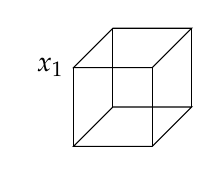
\begin{tikzpicture}[]
	\path[draw] (0,0) -- (1,0) -- (1+1/2,1/2) -- (1/2,1/2) -- cycle;
	\path[draw] (0,-1) -- (1,-1) -- (1+1/2,-1/2) -- (1/2,-1/2) -- cycle;
	\path[draw] (0,0) -- (0,-1) ;
	\path[draw] (1,0) -- (1,-1) ;
	\path[draw] (1+1/2,1/2) -- (1+1/2,-1/2) ;
	\path[draw] (1/2,1/2) -- (1/2,-1/2) ;
	\node[anchor = east] at (0,0) { $x_1 $ };
\end{tikzpicture}
\end{center}
\begin{proof}
If $x_1, \hdots , x_n  $ are linearly dependent, the Hadamard
inequality is trivial, suppose for the sequel that
$x_1, \hdots , x_n  $ are linearly independent, 
in other words
$\left( x_1, \hdots , x_n  \right) $ constitutes a basis 
of $\RR ^n  $, We use the Gram-Schmidtz process to transform
$\left( x_1, \hdots , x_n  \right) $ to an orthogonal basis
$\left( y_1, \hdots , y_n  \right) $ of $\RR ^n  $.

By The Gram-Schmidtz, there exist $\al_{ij}\in  \RR  
\left( 1 \leq j <  i \leq n \right)$ 
such that the vectors $y_1, \hdots , y_n  $ of $\RR ^n  $ defined by
\[
\begin{cases}
y_1 = x_1 \\
y_2 = x_2 + \al_{21} x_1 \\
y_3 = x_3 + \al_{31} x_1 + \al_{32} x_2 \\
\vdots \\
y_n = x_n + \al_{n1}x_1 + \al_{n2} x_2 + \hdots  + 
\al_{n, n-1} x_{n-1}
\end{cases}
\]
are pairwise orthogonal, by putting the condition 
in addition for $i,j \in \left\{ 1, \hdots , n \right\} $  
\[
\al_{i,j} = 
\begin{cases}
1 \\
0
\end{cases}
\begin{gathered}  
 i = j\\ 
 i < j
\end{gathered}
\quad 
\text{ and } 
\quad 
T = \left( \al_{i,j} \right)_{1 \leq i,j \leq n}
\in  \mathcal{M} (\RR ) 
\]
Which is a linear transformation with diagonal entries all equal to
$1$, as its non singular, 
specifically the system can be rewritten as 
\[
	\begin{pmatrix}
		y_1 \\
		y_2 \\
		\vdots \\
		y_n \\
	\end{pmatrix} = 
	\text{ \large $T $ \normalfont} 
	\begin{pmatrix}
		x_1 \\
		x_2 \\
		\vdots  \\
		x_n  \\
	\end{pmatrix}
\]
which gives 
\[
\begin{pmatrix}
	x_1 \\
	x_2 \\
	\vdots   \\ 
	 x_{n}\\
\end{pmatrix}
= 
\text{ \large $T^{-1}$ \normalfont} 
\begin{pmatrix}
       y_1 \\
	 y_{2}\\
	\vdots  \\
	y_{n} \\
\end{pmatrix}
\]
$T^{-1} $ as $(T)  $ is lower triangular with diagonal 
entries all equal to $1$, now let 
\[
	\left( \bb _{i,j} \right)_{1 \leq i,j \leq n} = 
	T^{-1} \quad 
	\bb _{i,j} = 
	\begin{cases}
	1  \\
	0
	\end{cases}
	\begin{gathered}  
	 i = j\\ 
	 j < j
	\end{gathered}
\]

and we have 
\[
\begin{cases}
x_1 = y_1 \\
x_2 = y_2 + \bb_{21}y_1 \\
x_3 = y_3 + \bb_{31} y_1 + \bb _{32} y_2 \\
\vdots \\
x_{n} = y_1 + \bb _{n1}y_1 + \hdots + \bb _{n, n-1} y_{n-1} \\
\end{cases}
\]
Now, since the determinant is an alternating multi linear form
then we desire from the above system, that 
\[
det(x_1, \hdots , x_n )  = 
det (y_1, \hdots , y_n )  
\]
Next, by the pythagorean theorem, we have
according to the system, the fact that $y_{i}'s$ are all pairwise orthogonal,
we get that : 

\[
\begin{cases}
	\| x_1 \| ^2  = \| y_1 \| ^2  \\
	\| x_2 \| ^2  = 
	\| y_2 \| ^2  + \bb_{21}^2 
	\| y_1 \| ^2   \geq \| y_2 \| ^2 
	\\  
	\| x_3 \| ^2 = 
	\| y_3 \| ^2 + \bb_{31}^2 \| y_1 \| ^2  + 
	\bb_{32}^2 \| y_2 \| ^2  
	\geq \| y_3 \| ^2 
	\\
	\vdots \\
	\| x_1 \| ^2  = 
	\| y_1 \| ^2  + \bb_{n1}^2  
	\| y_1 \| ^2 +   \hdots +
	\bb_{n,n-1}^2  \| y_{n-1} \| ^2  
	\geq \| y_n  \| ^2 
\end{cases}
\]
hence we get 
\[
	\| x_1 \| ^2 \cdot 
	\| x_2 \| ^2  \cdot \hdots 
	\| x_n  \|  ^2  \geq 
	\| y_1 \| ^2  \cdot  \| y_2 \| ^2 
	 \hdots   \| y_n \| ^2 
\]
that is 
\[
\| x_1 \| \cdot  \| x_2 \| \hdots \| x_n  \|  
\geq 
\| y_1 \| \cdot  \| y_1 \|  
\hdots  
\| y_n  \| 
\]
now, we are goin to show that 
\[
	\left| det(y_1, \hdots , y_n )  \right| 
	= 
	\| y_1 \| \cdot \| y_2 \|  \hdots 
	\| y_n  \| 
\]
Let $A = \left( y_1|y_2| \hdots| y_n  \right)  
\left( \in  \mathcal{M}_{n} (\RR )  \right)$, 
so 
\[
A^{T} = 
\begin{pmatrix}
	y_1^{T} \\
	\hline y_2^{T} \\
	\hline \vdots  \\
	\hline y_n ^{T} \\
\end{pmatrix}
\]

hence
\[
A^{T} A = 
\begin{pmatrix}
	y_1^{T} \\
	\hline y_2^{T} \\
	\vdots  \\
	\hline y_n ^{T} \\
\end{pmatrix}
\begin{pmatrix}
	 y_1|& y_2|  & \hdots|   & y_n   \\
\end{pmatrix}
\]
which equals
\[
	\begin{pmatrix}
		 \left\langle 
		 y_1, y_1\right\rangle & \hdots  & 
		 \left\langle y_1,y_n  \right\rangle \\
		\vdots  &  \ddots &  \vdots \\
		\left\langle y_n ,y_1 \right\rangle  & \hdots 
						     & 
		\left\langle y_{n},y_{n} \right\rangle \\
	\end{pmatrix}
	= 
	\begin{pmatrix}
		\| y_1 \| ^2  & \hdots  & (0)  \\
		\vdots  & \ddots  & \vdots  \\
		(0)  & \hdots  & \| y_n  \|^2   \\
	\end{pmatrix}
\]

so \[
A ^{T} A = 
diag (\| y_1 \| ^2 , \hdots , \| y _n  \| ^2 ) 
\]
then by taking the determinants
\[
	\left( detA \right)^2  = 
	\| y_1 \| ^2  \hdots  \| y _n   \| ^2 
\]
then 
\[
\left| det(A)  \right| = 
\| y_1 \| \hdots  \| y_n  \| 
\]
i.e 
\[
det (y_1, \hdots , y_n ) = 
\| y_1 \| \hdots  \| y_n  \| 
\]
confirming the formula, now we have according to 
1 ,2 and 3
\begin{align*}
	\left| det(x_1, \hdots , x_n   )  \right| & 
	= 
	\left| det(y_1, \hdots , y_n )  \right| \\
						  &=
						 \| y_1 \| 
		\| y_2 \|  \hdots  \| y_n  \| \\
	&= 
	\| x_1 \|  \cdot \| x_2 \|  \hdots 
	\| x_n  \| 
\end{align*}
as required, in addition the equlaity 
\[
	\left| det(x_1, \hdots  x_n )  \right| =
	\| x_1 \| \| x_2 \|  \hdots 
	\| x  _n \|  
\]
hold if and only if 
\[
	\| y_1 \| \hdots \| y_n  \|  = 
	\| x_1 \|  \hdots \| x _n  \| 
\]
but this equivalent according to $3 $ to 
$\| x_{i} \| = \| y_{i} \|  $  
for all $i $, which is equivalent to $\bb_{i,j}= 0 $  
for all $i > j $ , that is $T = I_{n} $ which is
equivalent to 
\[
\left( y_1, \hdots , y_n  \right) =
\left( x_1, \hdots , x_n  \right)
\]
which holds if and only if $x_1, \hdots , x_n  $  are
pairwsie orthogonal, the proof is complete
\end{proof}
% \end{document}

